%!BIB program=biber

\documentclass{article} %类型为文章
\usepackage[UTF8]{ctex} %中文编码宏
\usepackage[hidelinks]{hyperref} %超链接宏
\usepackage{geometry} %页面控制宏
\usepackage{fancyhdr} %页眉页脚宏
\usepackage{lastpage} %总计页的宏
\usepackage{color} %颜色控制宏
\usepackage{graphicx} %图片插入宏
\usepackage{subfigure} %子图插入宏
\usepackage{diagbox} %表格斜线宏
\usepackage{multirow} %纵向合并宏
\usepackage{makecell} %表格换行宏
\usepackage{amsmath} %公式插入宏
\usepackage{cases}
\usepackage{unicode-math} %公式样式宏
\usepackage{algorithm2e} %伪代码宏
\usepackage{gbt7714} %国标引用宏
\usepackage{url} %网页链接宏
\usepackage{doi} %doi号宏

\usepackage{listings}

\definecolor{dkgreen}{rgb}{0,0.6,0}
\definecolor{gray}{rgb}{0.5,0.5,0.5}
\definecolor{mauve}{rgb}{0.58,0,0.82}
\lstset{frame=tb,
  language=Python,
  aboveskip=3mm,
  belowskip=3mm,
  showstringspaces=false,
  columns=flexible,
  basicstyle={\small\ttfamily},
  numbers=left,%设置行号位置none不显示行号
  %numberstyle=\tiny\courier, %设置行号大小
  numberstyle=\tiny\color{gray},
  keywordstyle=\color{blue},
  commentstyle=\color{dkgreen},
  stringstyle=\color{mauve},
  breaklines=true,
  breakatwhitespace=true,
  escapeinside=``,%逃逸字符(1左面的键),用于显示中文例如在代码中`中文...`
  tabsize=4,
  extendedchars=false %解决代码跨页时,章节标题,页眉等汉字不显示的问题
}

\geometry{a4paper,left=2cm,right=2cm,top=2cm,bottom=2cm,headsep=0.5cm,footskip=1cm} %设置页边距和页眉页脚距离
\pagestyle{fancy} %设置页面样式
\fancyhf{} %开启页眉页脚
\lhead{计算物理数值报告} %设置左侧页眉为作者
\rhead{Sichuan University 四川大学} %设置右侧页眉为机构
\cfoot{第\thepage 页 \quad 共 \pageref{LastPage} 页} %设置居中页脚为页码

\linespread{1.2} %行距
\setlength{\parskip}{0.5em} %段落间距
\setlength{\parindent}{2em} %缩进距离

\setmathfont{Cambria Math} %设置数学公式样式
\bibliographystyle{gbt7714-numerical} %设置参考文献样式

\title{考虑带电粒子的电磁场对粒子本身反作用下\\带电粒子在匀强磁场中低速运动\\的数值模拟报告} %设置标题
\author{欧纪阳\footnote{E-mail: Julian-OU@outlook.com} 2019141220016\quad 赵春丽 2019141220081\\ 张凌凯 2019141220032\quad 苗森 2019141220028\quad 马卓瑜 2019141220045\\ \textit{College of Physics, Sichuan University, Chengdu 610064, China}} %设置作者
\date{\today} %设置日期

\begin{document}
\maketitle %插入标题
\begin{abstract}
  带电粒子与电磁场是相互作用的,一方面带电粒子激发电磁场,另一方面电磁场又对电荷有反作用,要完全解决带电粒子与电磁场系统的动力学问题,必须把两者直接的相互作用同时考虑。当考虑电带电粒子产生的辐射时,一部分能量和动量被电磁场带着,因此粒子的运动必然受到阻尼,在匀强磁场中的不再做圆周运动。本文将试图探究考虑带电粒子的电磁场对粒子本身的相互作用,即考虑辐射阻尼时粒子在匀强磁场中的运动,并在Python中使用龙格-库塔方法以及Mathematica进行数值模拟。\\
  \textbf{关键词:}电动力学 \quad 电磁辐射 \quad 辐射阻尼 \quad 自身场 \quad 初值问题 \quad Python \quad Mathematica
\end{abstract}

\section{介绍}
在电磁学中,带电粒子在恒定电磁场中运动,会受到电场力与洛伦兹力的作用。当只存在匀强磁场时,根据带电粒子初速度的不同,粒子将做匀速圆周运动或者保持半径不变的螺旋运动,前者粒子在延磁场方向上不具有速度,后者则在该方向上具有速度。

而在学习了电动力学之后,应该明白在实际情况中,粒子的运动会辐射电磁场,一部分能量和动量被电磁场带着,因此粒子的运动必然受到阻尼。因此粒子的运动不是单纯被外场作用力决定的,粒子所激发的场对粒子本身也有作用力,为了完全解出粒子的运动,必须在粒子的动力学方程中除了包含除该粒子本身以外的场产生的电场力和洛伦兹力以外,还必须包含该粒子自身产生的辐射场的反作用力,即辐射阻尼力。

在这篇文章中,我们报告了计算带电粒子在包含自身辐射场的电磁场中低速运动的方法,并使用Python进行数值计算。在本文的第二部分中,将讨论计算辐射阻尼的方法;本文的第三部分将会介绍数值模拟的方法;不考虑辐射阻尼的数值模拟的结果将展示在本文的第四部分;我们最后在第五部分中利用Mathematica讨论存在辐射阻尼的情况。

本文的相关代码已上传至GitHub公开库\url{https://github.com/812610357/Electrodynamics}。

\section{理论}
在这一部分中将会补充一些电动力学知识,讨论从推迟势到电偶极辐射的功率,再到使用辐射功率推到辐射阻尼的方法,得到带电粒子在电磁场中的运动方程。

\subsection{电磁场的推迟势}
把洛伦兹规范条件
\begin{align*}
  \nabla \cdot \pmb{A}+\frac{1}{c^2}\frac{\partial \varphi}{\partial t}=0
\end{align*}
以及用矢势$\pmb{A}$、标势$\varphi$表示的磁场、电场表示式
\begin{align*}
  \pmb{B} & =\nabla \times \pmb{A} & \pmb{E} & =-\frac{\partial \pmb{A}}{\partial t}-\nabla \varphi
\end{align*}
带入麦克斯韦方程组中
\begin{align*}
  \nabla \times \pmb{E} & =-\frac{\partial \pmb{B}}{\partial t} & \nabla \cdot \pmb{E} & =\frac{\rho}{\varepsilon_0} & \nabla \times \pmb{B} & =\mu_0 \varepsilon_0\frac{\partial \pmb{E}}{\partial t}+\mu_0 \pmb{J} & \nabla \cdot \pmb{B} & =0
\end{align*}
可以得到达朗贝尔方程
\begin{align*}
  \nabla^2 \pmb{A}-\frac{1}{c^2}\frac{\partial^2 \pmb{A}}{\partial t^2} & =-\mu_0\pmb{J} & \nabla^2 \varphi-\frac{1}{c^2}\frac{\partial^2 \varphi}{\partial t^2} & =-\frac{\rho}{\varepsilon_0}
\end{align*}
分别求解后可以得到推迟势公式
\begin{align}
  \pmb{A}(\pmb{x},t) & =\frac{\mu_0}{4\pi}\int_V \frac{\pmb{J}\left(\pmb{x}',t-\frac{r}{c} \right)}{r} \,\mathrm{d}V' & \varphi(\pmb{x},t) & =\frac{1}{4\pi\varepsilon_0}\int_V \frac{\rho\left(\pmb{x}',t-\frac{r}{c} \right)}{r} \,\mathrm{d}V' \label{e1}
\end{align}
以上两式表明电磁作用具有一定的传播速度,空间某点$\pmb{x}$在时刻$t$的场值不是依赖于同一时刻的电荷电流分布,而是决定于较早时刻
\begin{align*}
  t'=t-\frac{r}{c}
\end{align*}
的电荷电流分布。
\subsection{低速运动粒子的辐射场}
对带电粒子来说$\pmb{J}=\rho \pmb{v}$,其中$\pmb{v}$为粒子在辐射时刻$t'$的速度,由(\ref{e1})式可知势依赖于粒子的速度$\pmb{v}$,而不依赖于加速度$\dot{\pmb{v}}$,因此可以取一个在粒子辐射时刻相对静止的参考系$\tilde{\Sigma}$,则在$\tilde{\Sigma}$观察$\left( \tilde{\pmb{x}},\tilde{t} \right)$上势的瞬间值为
\begin{align*}
  \tilde{\pmb{A}} & =0 & \tilde{\varphi} & =\frac{q}{4\pi\varepsilon_0 \tilde{r}}
\end{align*}
其中$\tilde{r}=c\left( \tilde{t}-\tilde{t}' \right)$为$\tilde{\Sigma}$上观察的粒子与场点的距离。运用洛伦兹变换把势变换回原参考系$\Sigma$中
\begin{align*}
  \pmb{A} & =\frac{\pmb{v}\tilde{\varphi}}{c^2\sqrt{1-\frac{v^2}{c^2}}} = \frac{1}{\sqrt{1-\frac{v^2}{c^2}}}\frac{q\pmb{v}}{4\pi\varepsilon_0 c^2\tilde{r}} & \varphi & =\frac{\tilde{\varphi}}{\sqrt{1-\frac{v^2}{c^2}}}=\frac{1}{\sqrt{1-\frac{v^2}{c^2}}}\frac{q}{4\pi\varepsilon_0 \tilde{r}}
\end{align*}
其中$\tilde{r}$任然是$\tilde{\Sigma}$上观察到的距离,用洛伦兹变换将其改写为$\Sigma$上的距离
\begin{align*}
  \tilde{r}=\left( \tilde{t}-\tilde{t}' \right)=\frac{c\left( t-t' \right)-\frac{\pmb{v}}{c}\cdot\left( \pmb{x}-\pmb{x}' \right)}{\sqrt{1-\frac{v^2}{c^2}}}=\frac{r-\frac{\pmb{v}}{c}\cdot \pmb{r}}{\sqrt{1-\frac{v^2}{c^2}}}
\end{align*}
因此得到势在$\Sigma$下的表达式
\begin{align}
  \pmb{A} & =\frac{q\pmb{v}}{4\pi\varepsilon_0 c^2 \left( r-\frac{\pmb{v}}{c}\cdot \pmb{r} \right)} & \varphi & =\frac{q}{4\pi\varepsilon_0 \left( r-\frac{\pmb{v}}{c}\cdot \pmb{r} \right)} \label{e2}
\end{align}
因为当低速运动$v\ll c$时有
\begin{align*}
  \frac{\partial t'}{\partial t} &=\frac{r}{r-\frac{\pmb{v}\cdot \pmb{r}}{c}}=1 & \nabla t'&=-\frac{r}{c\left( r-\frac{\pmb{v}\cdot \pmb{r}}{c} \right)}=-\frac{\pmb{r}}{cr}=-\frac{-\pmb{e}_r}{c}
\end{align*}
把势公式(\ref{e2})式对时空坐标微分得
\begin{align*}
  \pmb{B}&=\nabla \times \pmb{A}=\nabla \times \left. \pmb{A} \right|_{t'=const.}+\nabla t'\times \frac{\partial \pmb{A}}{\partial t'}=\frac{q\pmb{v}\times\pmb{r}}{4\pi\varepsilon_0 c^2 r^3}-\frac{\pmb{r}}{cr}\times\frac{q\dot{\pmb{v}}}{4\pi\varepsilon_0 c^2 r}=\frac{q\pmb{v}\times\pmb{r}}{4\pi\varepsilon_0 c^2 r^3}-\frac{q\dot{\pmb{v}}\times\pmb{r}}{4\pi\varepsilon_0 c^3 r^2}\\
  \pmb{E}&=-\frac{\partial \pmb{A}}{\partial t}-\nabla \varphi=-\frac{\partial t'}{\partial t}\frac{\partial \pmb{A}}{\partial t'}-\nabla \left. \varphi \right|_{t'=const.}-\nabla t'\frac{\partial \varphi}{\partial t'}=\frac{q{\pmb{r}}}{4\pi\varepsilon_0 r^3}-\frac{q\dot{\pmb{v}}}{4\pi\varepsilon_0 c^2 r}+\frac{\pmb{r}}{cr}\frac{q\dot{{\pmb{v}}}\cdot \pmb{r}}{4\pi\varepsilon_0 c r^2}=\frac{q{\pmb{r}}}{4\pi\varepsilon_0 r^3}+\frac{q\pmb{r}\times\left( \pmb{r}\times\dot{\pmb{v}} \right)}{4\pi\varepsilon_0 c^2 r^3}
\end{align*}
其中与$r$成反比的项为辐射电磁场
\begin{align*}
  \pmb{B}&=\frac{q\dot{\pmb{v}}\times \pmb{r}}{4\pi\varepsilon_0 c^3 r^2}=\frac{q}{4\pi\varepsilon_0 c^3}\dot{\pmb{v}}\times \pmb{e}_r&
  \pmb{E}&=\frac{q\dot{\pmb{v}}\times \pmb{r}}{4\pi\varepsilon_0 c^3 r^2}=\frac{q}{4\pi\varepsilon_0 c^2}\pmb{e}_r\times\left( \pmb{e}_r\times\dot{\pmb{v}} \right)
\end{align*}
于是可以得到辐射能流密度以及辐射总功率
\begin{align*}
  \pmb{S}&=\pmb{E}\times\pmb{B}=\frac{q^2\dot{\pmb{v}}^2}{16\pi^2\varepsilon_0 c^3 r^2}\sin^2{\Theta}\pmb{e}_r&
  P&=\oint \pmb{S}\cdot\pmb{e}_r r^2 \,\mathrm{d}\Omega=\frac{q^2\dot{\pmb{v}}^2}{6\pi\varepsilon_0 c^2} 
\end{align*}
其中$\Theta$表示$\pmb{r}$与$\dot{\pmb{v}}$的夹角。
\subsection{辐射阻尼力与运动方程}
当带电粒子受外力作用二加速时,粒子将辐射出电磁波,把部分能量辐射出去,因而粒子受到一个阻尼力,设$\pmb{F}_e$表示外力,$\pmb{F}_s$代表粒子激发的场对粒子本身的反作用力,即辐射阻尼力,则粒子的运动方程为
\begin{align*}
  m\dot{\pmb{v}}=\pmb{F}_e+\pmb{F}_s
\end{align*}
其中辐射阻尼力对粒子所作的负功率应等于辐射功率
\begin{align}
  \pmb{F_s}\cdot\pmb{v}=-P=-\frac{q^2 \dot{\pmb{v}}^2}{6\pi \varepsilon_0 c^3} \label{e3}
\end{align}
(\ref{e3})式中,粒子在某一瞬间时的速度$\pmb{v}$与加速度$\dot{\pmb{v}}$一般是不相关的量,(\ref{e3})式右边不能表示为一个力乘上速度$\pmb{v}$的形式,因此(\ref{e3})式不可能对每一瞬间成立,但是在粒子作准圆周运动时,当粒子运动一周后,粒子附近的场回到原来的状态,可以考虑使用平均阻尼效应,即(\ref{e3})式对一周期积分是成立的
\begin{align*}
  \int_{t_0}^{t_0+T} \pmb{F}_s \cdot \pmb{v} \,\mathrm{d}t=\int_{t_0}^{t_0+T} -\frac{q^2 \dot{\pmb{v}}^2}{6\pi \varepsilon_0 c^3} \,\mathrm{d}t=\left. -\frac{q^2}{6\pi \varepsilon_0 c^3}\dot{\pmb{v}}\cdot\pmb{v}\right| _{t_0}^{t_0+T}+\int_{t_0}^{t_0+T} \frac{q^2 \ddot{\pmb{v}}\cdot\pmb{v}}{6\pi \varepsilon_0 c^3} \,\mathrm{d}t
\end{align*}
其中第一项为零,因为当粒子运动一周后,$\dot{\pmb{v}}$与$\pmb{v}$回到原值,因此辐射阻尼力可取
\begin{align*}
  \pmb{F}_s=\frac{q^2 \ddot{\pmb{v}}}{6\pi \varepsilon_0 c^3}
\end{align*}
于是便得到了带电粒子在匀强磁场中的运动方程
\begin{align}
  m\dot{\pmb{v}}=q\pmb{v}\times \pmb{B}+\frac{q^2 \ddot{\pmb{v}}}{6\pi \varepsilon_0 c^3} \label{e4}
\end{align}
\section{方法}
由于题目所给的带电粒子质量和电荷的数量级导致辐射阻尼力的数量级为$10^{-14}$次方,小于机器精度,因此在使用Python编写时将不考虑辐射阻尼力,但是在报告的第四部分中,将给出使用Mathematica求解的结果对比。

在上一部分中,通过推导得到了带电粒子的运动方程(\ref{e4})式去掉辐射阻尼力后为一个二阶矢量偏微分方程,可以改写为三个标量方程
\begin{align*}
  m\ddot{\pmb{r}}=q\dot{\pmb{r}}\times\pmb{B}\Rightarrow
  \begin{cases}
    m\ddot{r}_x=\dot{r}_y B_z-\dot{r}_z B_y\\
    m\ddot{r}_y=\dot{r}_z B_x-\dot{r}_x B_z\\
    m\ddot{r}_z=\dot{r}_x B_y-\dot{r}_y B_x\\
  \end{cases}
\end{align*}
通过重新定义变量,使上述三个二阶常微分方程变为六个一阶常微分方程
\begin{align}
  \begin{cases}
    w_{x1}=r_x,\, w_{x2}=\dot{r}_x\\
    w_{y1}=r_x,\, w_{y2}=\dot{r}_y\\
    w_{z1}=r_x,\, w_{z2}=\dot{r}_z
  \end{cases}
  \Rightarrow
  \begin{cases}
    w'_{x1}=w_{x2},\, w'_{x2}=w_{y2} B_z-w_{z2} B_y\\
    w'_{y1}=w_{y2},\, w'_{y2}=w_{z2} B_x-w_{x2} B_z\\
    w'_{z1}=w_{z2},\, w'_{z2}=w_{x2} B_y-w_{y2} B_x
  \end{cases}
  \label{e5}
\end{align}
对以上六个方程组成的方程组,应用4阶龙格-库塔方法进行求解,具体算法如Algorithm\ref{A1}所示。
\begin{algorithm}[t]
  \LinesNumbered
  \KwIn{$f$:导数对应的函数\newline
      $t$:求解范围\newline
      $h$:求解步长\newline
      $w_0$:$t=0$时的初值}
  $n$=int($t/h$)\\
  $t_0=0$\\
  \For{$i=0,1,2,\cdots,n-1$}{
    $s1 = f(t_i, w_i)$\\
    $s2 = f(t_i + h/2, w_i + s1*h/2)$\\
    $s3 = f(t_i + h/2, w_i + s2*h/2)$\\
    $s4 = f(t_i + h, w_i + s3*h)$\\
    $w_{i+1} = w_i + (s1 + 2*s2 + 2*s3 + s4)*h/6$\\
    $t_{i+1}=t_i+h$
  }
  \KwOut{$t_0,t_1,\cdots,t_n$:自变量序列\newline
      $w_0,w_1,\cdots,w_n$:方程组的解}
  \caption{4阶龙格库塔方法}
  \label{A1}
\end{algorithm}
\section{结果}
利用Python编写4阶龙格-库塔方法,代入(\ref{e5})式中的方程组,并设置初始条件为
\begin{align*}
  \begin{cases}
    w_{x1}=-3,w_{x2}=1\\
    w_{x1}=3,w_{x2}=2\\
    w_{x1}=0,w_{x2}=0.1
  \end{cases}
\end{align*}
时间设置为$t=5$,步长设置为$h=0.001$进行求解,粒子的运动轨迹如图\ref{A1}(a)所示。
\begin{figure}[h]
  \centering
  \subfigure[粒子的运动轨迹]{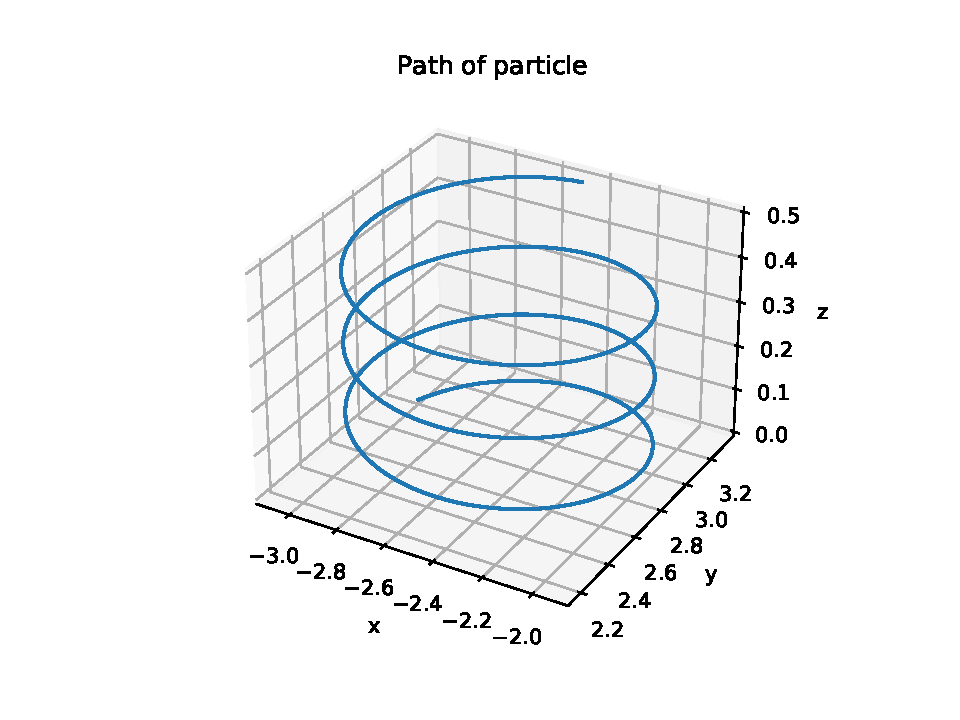
\includegraphics[width=8cm]{p.pdf}}
  \subfigure[误差曲线]{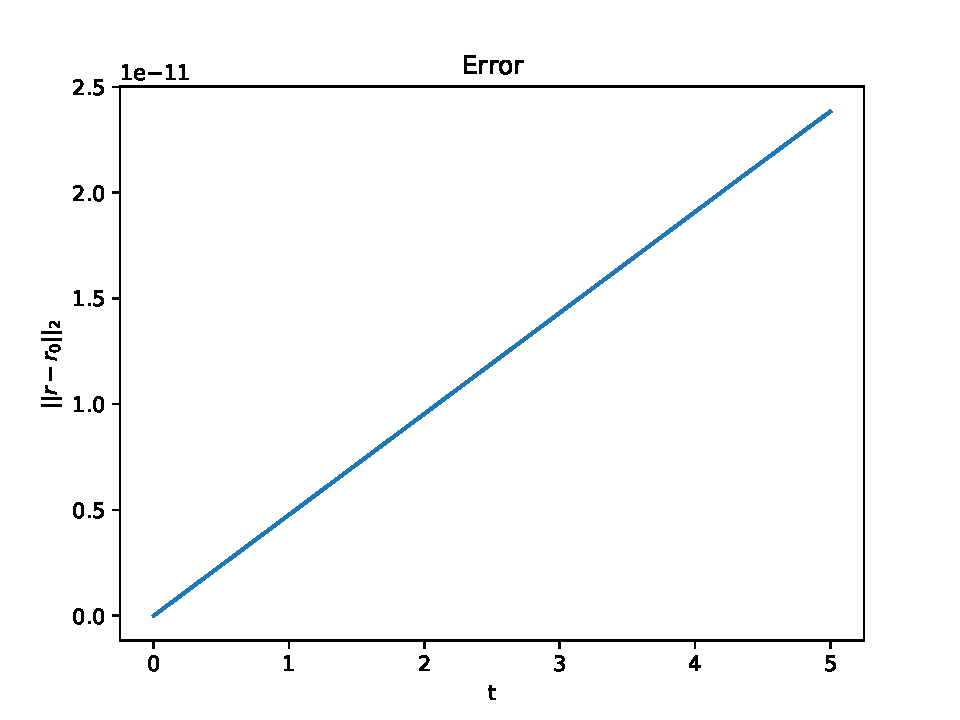
\includegraphics[width=8cm]{e.pdf}}
  \caption{数值计算结果}
  \label{P1}
\end{figure}
该问题具有解析解,按以上初始条件下的解析解如(\ref{e6})式,计算二范数误差绘制,如图\ref{A1}(b)所示,计算得到的粒子距离原点的最小距离约为3.15872071,解析解所给出的最小距离为3.15871956。
\begin{align}
  \begin{cases}
    x=\frac{1}{4}(-2\cos{4t}+\sin{4t}-10)\\
    y=\frac{1}{4}(\cos{4t}+2\sin{4t}+11)\\
    z=0.1t
  \end{cases}
  \label{e6}
\end{align}

\section{讨论}
由于数量级差别巨大,无法在Python中利用4阶龙格-库塔方法进行求解,在此利用商业数学软件Mathematica求解微分方程组进行求解,设置相同的初始条件,结果如图\ref{P2}所示。计算结果表明,阻尼力的存在使粒子的运动轨迹不再以圆轨道螺旋上升,而是做半径逐渐减小的螺旋上升运动,这是由于粒子运动辐射出电磁波,使其能量和动量损失所造成的。但是由于辐射功率较低,导致辐射阻尼力远小于洛伦兹力,只有在粒子长时间运动后其运动的半径才会有明显的变化。
\begin{figure}[t]
  \begin{center}
    \subfigure[$t=0\sim 5$时的粒子运动轨迹]{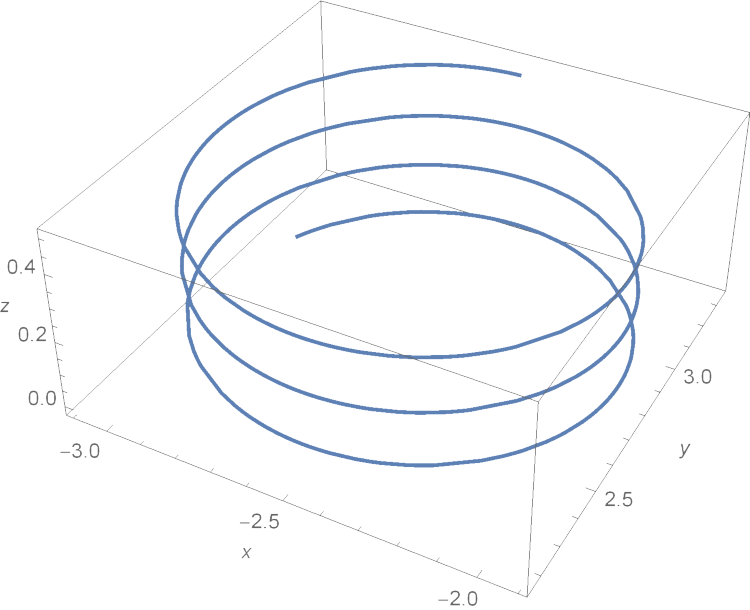
\includegraphics[width=8cm]{1.pdf}}
    \subfigure[$t=9995\sim 10000$时的粒子运动轨迹]{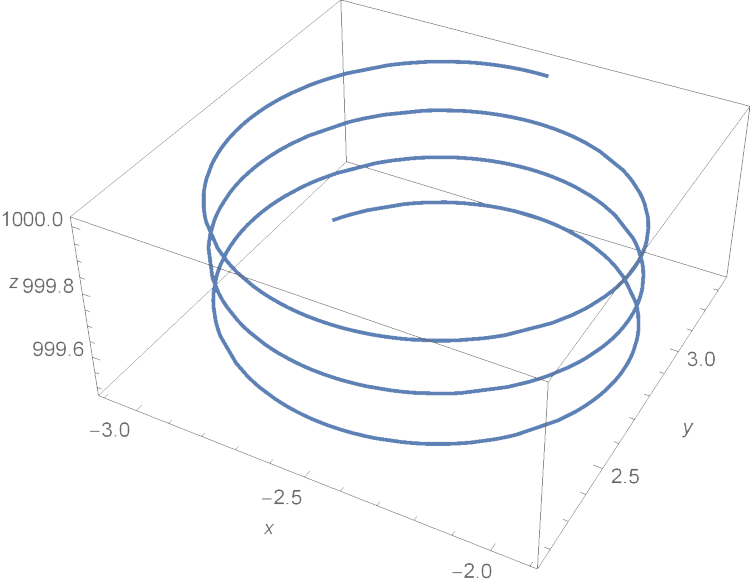
\includegraphics[width=8cm]{2.pdf}}
    \subfigure[$t=0\sim 10$时的计算结果对比图]{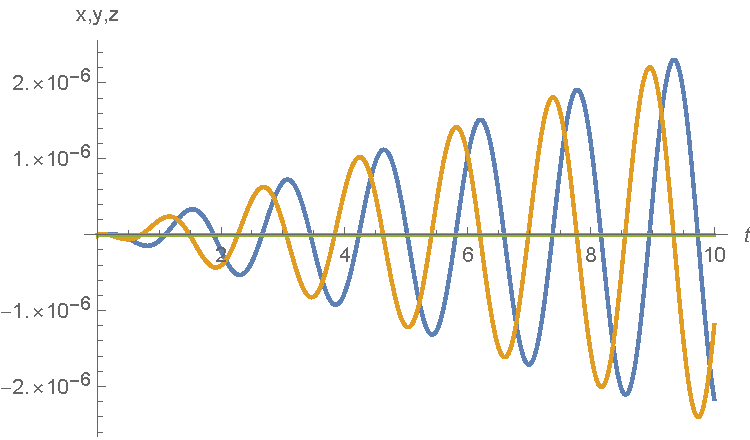
\includegraphics[width=8cm]{3.pdf}}
    \subfigure[$t=9998\sim 10000$时的计算结果对比图]{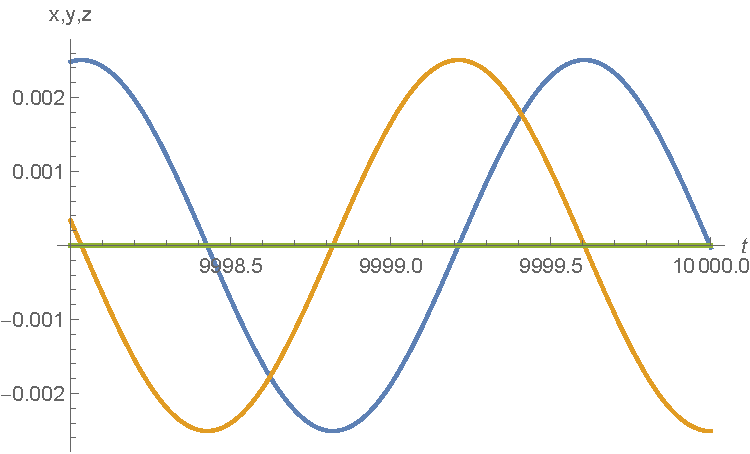
\includegraphics[width=8cm]{4.pdf}}
  \end{center}
  \quad (a)和(b)为不同时间的段的数值计算结果;(c)和(d)展示了不同时间段内,考虑了辐射阻尼与未考虑辐射阻尼的计算结果差异(用考虑了阻尼的计算结果减去未考虑的),蓝色线条表示$x$方向,橙色线条表示$y$方向,绿色线条表示$z$方向。
  \caption{Mathematica的求解结果}
  \label{P2}
\end{figure}
\section{鸣谢}
感谢以下基金对本工作的支持,国家自然科学基金:11875227,12047573,11875196;波谱与原子分子物理国家重点实验室开放基金:T151603
\begin{thebibliography}{12}
  [1] 郭硕泓,电动力学(第三版),高等教育出版社,2008. 6\newline
  [2] Sauer, T.,数值分析(原书第二版),工业出版社,2014. 10
\end{thebibliography}
\section*{附代码}
不考虑辐射阻尼的Python代码如下,原始代码文件以及Mathematica笔记本在附文件中可以找到。
\begin{lstlisting}
import numpy as np
import matplotlib.pyplot as plt

m = 1
q = 1
B = np.array([0, 0, 4])
r0 = np.array([-3, 3, 0])    # 初始位置
v10 = np.array([1, 2, 0.1])  # 初始速度
v20 = q*np.cross(v10, B)/m   # 初始加速度
y0 = np.append(r0, v10)

c = 2.99792458e8
epsilon = 8.854187817e-12
k = q**2/(6*np.pi*epsilon*c**3)


def f(t, x):
    x1 = x[:3]
    x2 = x[3:]
    s1 = x2
    s2 = q*np.cross(x2, B)/m
    s = np.append(s1, s2)
    return s


def RK4(f, t, h, y0):
    n = int(t/h)
    t = np.linspace(0, t, n+1)
    w = np.zeros((len(y0), n+1))
    w[:, 0] = np.array([y0])
    for i in range(n):
        s1 = f(t[i], w[:, i])
        s2 = f(t[i] + h/2, w[:, i] + s1*h/2)
        s3 = f(t[i] + h/2, w[:, i] + s2*h/2)
        s4 = f(t[i] + h, w[:, i] + s3*h)
        w[:, i+1] = w[:, i] + (s1 + 2*s2 + 2*s3 + s4)*h/6
    return t, w


t, r = RK4(f, 5, 1e-3, y0)
fig = plt.figure()
ax = fig.add_subplot(111, projection='3d')
ax.plot(r[0], r[1], r[2])
ax.set_xlabel('x')
ax.set_ylabel('y')
ax.set_zlabel('z')
ax.set_title('Path of particle')
plt.savefig('p.pdf')
plt.show()


def g(t):
    x = (-10 - 2*np.cos(4*t) + np.sin(4*t))/4
    y = (11 + np.cos(4*t) + 2*np.sin(4*t))/4
    z = 0.1*t
    return np.array([x, y, z])


r0 = g(t)
error = np.linalg.norm(r[:3]-r0, ord=2, axis=0)
plt.plot(t, error)
plt.title('Error')
plt.xlabel('t')
plt.ylabel('$||r-r_0||_2$')
plt.savefig('e.pdf')
plt.show()

print(np.min(np.linalg.norm(r[:3], ord=2, axis=0)))
\end{lstlisting}
\end{document}